%!TEX root = main.tex
\section{Synchronizability}\label{sec:criterion}

%In order to simplify the reasoning about the asynchronous semantics of a message passing system $\mathcal{S}$, 
We define a property called \emph{$k$-synchronizability}, for some $k>0$, which roughly, states that every execution of a message passing system $\mathcal{S}$ is ``equivalent'' to one which passes regularly through configurations where the message buffers are empty, and in between those configurations, the overall number of messages stored in the buffers is bounded by $k$ (where by ``equivalent'', we mean conflict-preserving permutation). We formalize this property as the equality between the set of traces generated by the asynchronous semantics and the set of traces generated by a particular semantics called \emph{$k$-synchronous} which allows precisely the kind of executions mentioned above.

\begin{figure}[t]
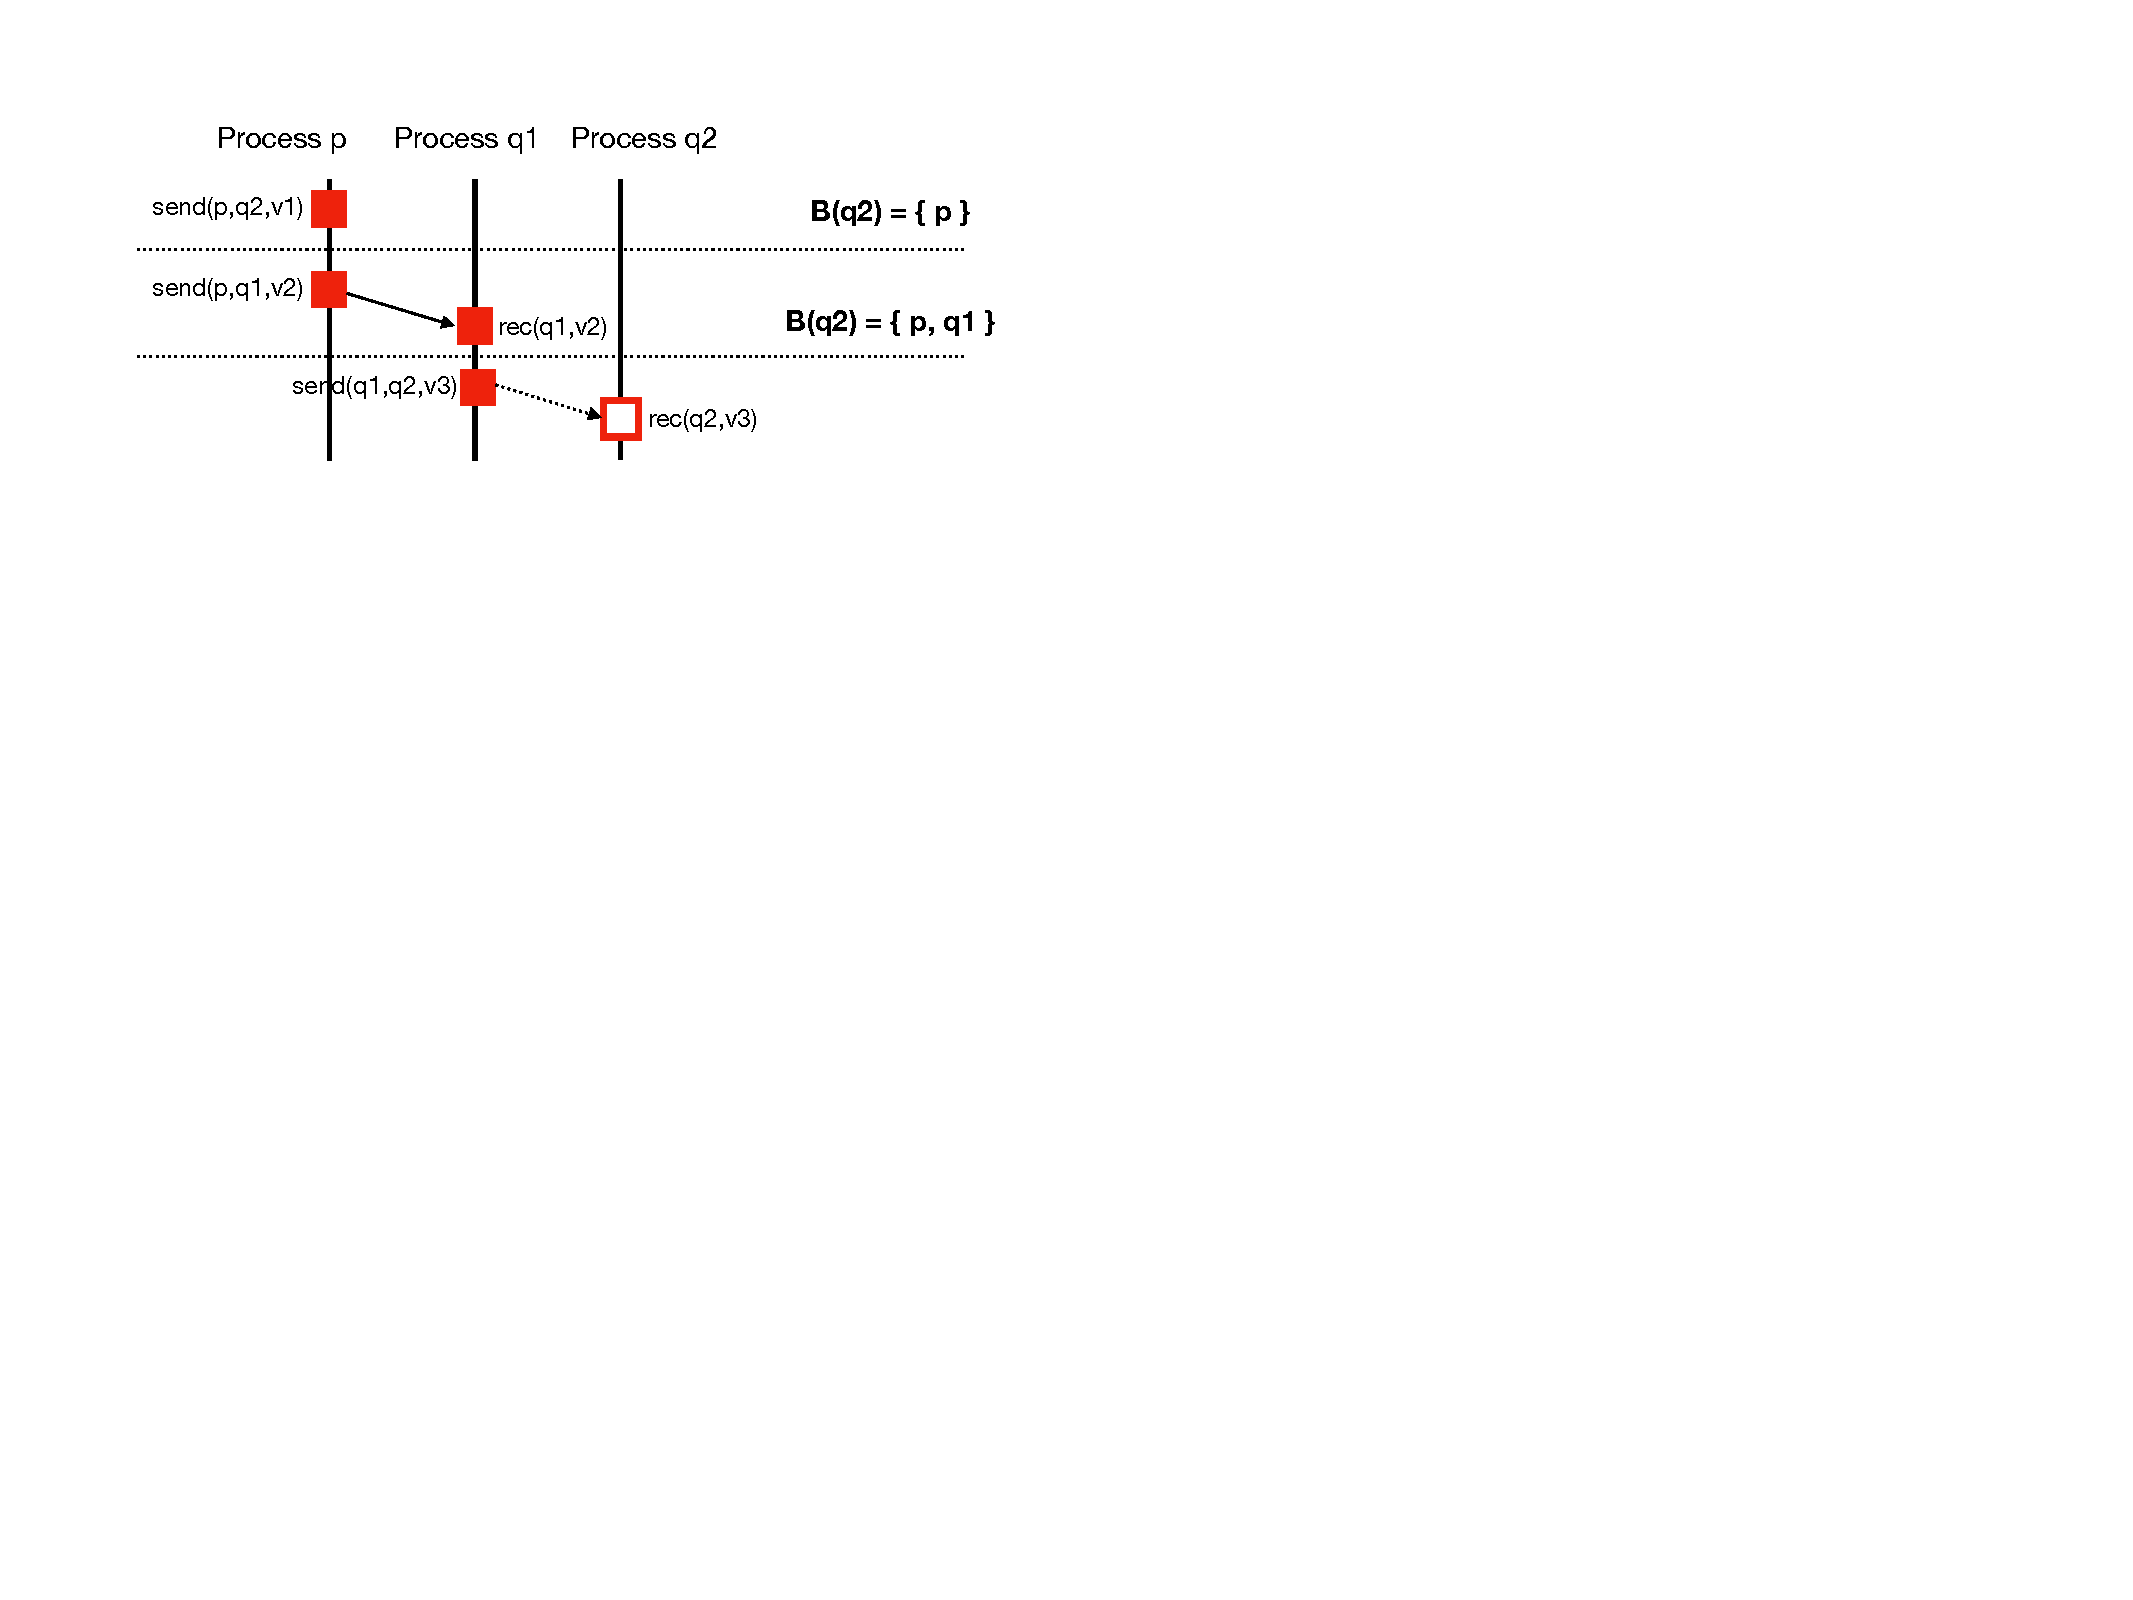
\includegraphics[width=8cm]{ex-blocking.pdf}
\caption{An execution of the $1$-synchronous semantics.}
\label{fig:ex-blocking}
\end{figure}

The $k$-synchronous semantics we define hereafter uses an extended version of the standard rendez-vous primitive where the message sent by a process is instantaneously received by the destination process. Roughly, in this extension, more than one process is allowed to send a message and a process can send multiple messages, but all these messages must be received before being allowed to send more messages. This primitive is called \emph{$k$-exchange} if the number of sent messages is smaller than $k$. Actually, to ensure that the $k$-synchronous semantics is prefix-closed (if it admits an execution, then it admits all its prefixes), we allow messages to be dropped during a $k$-exchange transition. For instance, the following execution 
\begin{align*}
\send{1}{p_1,q,\_}\ 
\send{2}{p_2,q,\_}\ 
\rec{1}{q,\_}\ 
\rec{2}{q,\_} 
\end{align*}
is an instance of a $2$-exchange and therefore admitted by the $2$-synchronous semantics. However, in order to ensure that the prefix without the last receive ($\rec{2}{q,\_}$) is also admitted, we allow $2$-exchange transitions to contain unmatched send actions. The presence of unmatched send actions must be constrained in order to ensure that the set of executions admitted by the $k$-synchronous semantics satisfies causal delivery. Consider for instance the execution in Figure~\ref{fig:ex-blocking} which can be produced by a sequence of $1$-exchanges. The receive action ($\reca{q_2,v_3}$) pictured as an empty box needs to be disabled in order to exclude violations of causal delivery. To this, the semantics tracks for each process $p$ a set of processes $B(p)$ from which it is forbidden to receive messages. Following the sequence of $1$-exchanges in this execution, the unmatched $\senda{p,q2,v1}$ disables any receive by $q2$ of a message sent by $p$ (otherwise, it will be even a violation of the FIFO semantics of $q2$'s buffer). Therefore, the first $1$-exchange results in $B(q2)=\{p\}$. The second $1$-exchange (the message from $p$ to $q1$) forbids $q2$ to receive any message from $q1$. Otherwise, this message will be necessarily causally related to $v1$, and receiving it will lead to a violation of causal delivery. Therefore, when reaching $\senda{q1,q2,v_3}$ the receive $\reca{q_2,v_3}$ is disabled because $q1\in B(q2)$.

%The standard rendez-vous primitive corresponds to the $1$-exchange. 
%The semantics allows messages to be dropped, but  TODO SAY THAT THIS IS RELATED TO AN IMPLICIT FIFO SEMANTICS FOR THE BUFFERS

\begin{figure} [t]
\footnotesize{
  \centering
  \begin{mathpar}
    \inferrule[$k$-exchange]{
      e\in S_{id}^*\cdot R_{id}^* \\ 
       |e| \leq 2\cdot k\\
%      \<msg>(a)\in [1,k]\mbox{ for every $a$ in $e$} \\
      (\vec{l},\vec{\epsilon})\xrightarrow{e} (\vec{l'},\vec{b}),\mbox{ for some $\vec{b}$}\\
            \forall s,r\in e.\ s\match r\implies\<proc>(s)\not\in B(\<dest>(s)) \\
       B'(q) = B(q) \cup \{p: \exists s\in e\cap S_{id}.\ ((\not\exists r\in e.\ s\match r)\land p = \<proc>(s)\land q=\<dest>(s)) \lor (\<proc>(s)\in B(q)\land \<dest>(s) = p)\}
    }{
      (\vec{l},B)
      \xRightarrow{e}{_k}
      (\vec{l'},B')
    }%\hspace{5mm}
    
%    \inferrule[drop]{
%      l\in \delta_p(\vec{l}_p,\senda{p,q,v}) \neq \emptyset
%    }{
%      (\vec{l},F)
%      \xRightarrow{\senda{p,q,v}}{_k}
%      (\vec{l}[\vec{l}_p\gets l],F\cup \{q\})
%    }%\hspace{5mm}
    
%    \inferrule[local]{ 
%      l\in \delta(\vec{l}_p,\epsilon) \neq \emptyset
%    }{
%      \vec{l},\vec{b}
%      \xrightarrow{\epsilon}
%      \vec{l}[\vec{l}_p\gets l],\vec{b}
%    }%\hspace{5mm}
  \end{mathpar}
  }
% \vspace{-5mm}
  \caption{The synchronous semantics of a message passing system $\mathcal{S}$. Above, $\vec{\epsilon}$ denotes a vector where all the components are $\epsilon$.
  %and for a sequence of indexed actions $e\in(S_{id}\cup R_{id})^*$, $\overline{e}$ denotes the sequence of \emph{actions} obtained from $e$ by removing message identifiers.
  %$\vec{b}[\vec{b}_q.\ \mathrm{add}(m)]$ denotes the vector of message buffers obtained from $\vec{b}$ by calling the method $\mathrm{add}(m)$ of the element of index $q$.
  }
  \label{fig:synch-sem}
%\vspace{-6mm}
\end{figure}

Formally, a configuration $c'=(\vec{l},B)$ in the synchronous semantics is a vector $\vec{l}$ of local states together with a function $B:\<Pids>->2^{\<Pids>}$. The transition relation $\Rightarrow_k$ is defined in Figure~\ref{fig:synch-sem}. A \textsc{$k$-exchange} transition corresponds to a sequence of transitions of the asynchronous semantics starting from a configuration with empty buffers. The sequence of transitions is constrained to be a sequence of at most $k$ sends followed by a sequence of receives. The receives are enabled depending on previous unmatched sends as explained above, using the function $B$.
The semantics defined by $\Rightarrow_k$ is called the $k$-synchronous semantics.

Executions and traces are defined as in the case of the asynchronous semantics, using $\Rightarrow_k$ for some fixed $k$ instead of $\rightarrow$. The set of executions, resp., traces, of $\mathcal{S}$ under the $k$-synchronous semantics is denoted by $\synchExec{\mathcal{S}}{k}$, resp., $\synchTr{\mathcal{S}}{k}$. The executions in $\synchExec{\mathcal{S}}{k}$ and the traces in 
$\synchTr{\mathcal{S}}{k}$ are called $k$-synchronous. 

%A trace $t\in \synchTr{\mathcal{S}}{k}$, for some $\mathcal{S}$, is called $k$-synchronous. 
An execution $e$ such that $tr(e)$ is $k$-synchronous is called $k$-synchronizable. We omit $k$ when it is not important. 

For a given system $\mathcal{S}$, the set of executions generated by $\mathcal{S}$ under the $k$-synchronous semantics is prefix-closed. Therefore, the set of $k$-synchronizable executions of a system $\mathcal{S}$ is also prefix-closed.

\begin{lemma}\label{lem:pref_closed}
For a system $\mathcal{S}$, let $e\in\asynchExec{\mathcal{S}}$ be a $k$-synchronizable execution. Then, every prefix of $e$ is $k$-synchronizable. 
\end{lemma}
%\begin{proof}
%%We have to show that every cycle in a prefix $e'$ of $e$ is good and of size at most $k$. 
%Since the conflict graph $CG_{tr(e')}$ is a subgraph of $CG_{tr(e)}$, every cycle in $CG_{tr(e')}$ occurs also in $CG_{tr(e)}$. Therefore, since all the cycles of $e$ are good and of size at most $k$, the same holds for all the cycles in $e'$.
%\end{proof}

As a direct consequence of Lemma~\ref{lem:undist}, we get that $k$-synchronizable and $k$-synchronous executions are undistinguishable up to conflict-preserving permutations.

\begin{lemma}\label{lem:zable_nous}
For every $k$-synchronizable execution $e$, there exists a permutation $e'$ of $e$ which is $k$-synchronous.
\end{lemma}


\begin{definition}\label{def:synchron}
A message passing system $\mathcal{S}$ is called \emph{$k$-synchronizable} when $\asynchTr{\mathcal{S}}=\synchTr{\mathcal{S}}{k}$.
\end{definition}

%As a consequence of Definition~\ref{def:synchron}, a system $\mathcal{S}$ is not $k$-synchronizable when it admits an execution $e$ (under the asynchronous semantics) which is not $k$-synchronous (i.e., its trace is not $k$-synchronous). Such an execution $e$ is called a \emph{violation to $k$-synchronizability}.

The following result shows that $k$-synchronizable systems reach exactly the same set of local state vectors under the asynchronous and the $k$-synchronous semantics. Therefore, any assertion checking or invariant checking problem for a $k$-synchronizable system $\mathcal{S}$ can be solved by considering the $k$-synchronous semantics instead of the asynchronous one. In particular, this implies that such problems are decidable for finite-state $k$-synchronizable systems~\footnote{A system is called \emph{finite-state} when the number of local states of every process is bounded.} whereas they are undecidable for arbitrary systems. The $k$-synchronous semantics of a finite-state system can be modeled by a finite-state labeled transition system since the message buffers are of bounded size.

\begin{theorem}
For a $k$-synchronizable message passing system $\mathcal{S}$, $\asynchSt{\mathcal{S}}=\synchSt{\mathcal{S}}{k}$.
\end{theorem}
\begin{proof}
Direct consequence of Lemma~\ref{lem:undist}.
\end{proof}

In addition to assertion/invariant checking, we show that the problem of detecting deadlocks in a $k$-synchronizable system can also be solved using the $k$-synchronous semantics instead of the asynchronous one. 
We consider several notions of deadlock: a configuration $c=(\vec{l},\vec{b})$ is called 
\begin{itemize}
	\item \emph{empty-buffer deadlock} when all the buffers are empty, there exists at least one process waiting for a message, and all the other processes are either in a final or receiving state, i.e., $\vec{b}=\vec{\epsilon}$, there exists $p\in\<Pids>$ such that $(\vec{l}_p,r,l')\in\delta_p$ for some $r\in R$, and for all $q\in \<Pids>$, $\vec{l}_q$ is receiving or final,
	\item \emph{orphan message configuration} when there is at least a non-empty buffer and each process is in a final state, i.e., $\vec{b}\neq\vec{\epsilon}$ and for all $p\in \<Pids>$, $\vec{l}_p$ is final,
	\item \emph{unspecified reception} when some process is prevented from receiving any message from its buffer, i.e., there exists $p\in\<Pids>$ such that $\vec{l}_p$ is receiving, and for all $\reca{p,v}\in R$, if $(\vec{l}_p,\reca{p,v},l')\in \delta_p$, for some $l'$, then $\vec{b}_p\not\in v\<Val>^*$.
\end{itemize}

We show that reachability of such configurations in the original asynchronous semantics can be reduced to reachability problems over the synchronous semantics, provided that the system is $k$-synchronizable. The constraints over the buffers of the asynchronous configurations are replaced by constraints over the executions (traces) of the synchronous semantics. For instance, an execution reaching an empty-buffer configuration is ``equivalent'' to a synchronous \emph{matched} execution where every sent message has been received (assuming $k$-synchronizability).

We extend the notion of empty-buffer deadlock to configurations of the synchronous semantics by removing the condition that the buffers are empty.

\begin{theorem}\label{th:deadlock1}
A $k$-synchronizable system $\mathcal{S}$ reaches an empty-buffer deadlock configuration under the asynchronous semantics iff the $k$-synchronous semantics of $\mathcal{S}$ admits a matched execution to an empty-buffer deadlock configuration.
\end{theorem}
\begin{proof}
We prove the only-if direction, the reverse being similar. 
Let $e$ be an execution in $\asynchExec{\mathcal{S}}$ to an empty-buffer deadlock configuration $(\vec{l},\vec{\epsilon})$. Since the buffers are empty, by the definition of the asynchronous semantics, we get that $e$ is matched. By $k$-synchronizability, there exists a permutation $e'$ of $e$ that belongs to $\synchExec{\mathcal{S}}{k}$. Then, by Lemma~\ref{lem:undist}, $e'$ is an execution to a configuration $(\vec{l},B)$, for some $B$, which finishes the proof.
\end{proof}

A configuration $(\vec{l},B)$ of the synchronous semantics is called \emph{final} when every local state $\vec{l}_p$ with $p\in\<Pids>$ is final. The proof of the following result is similar to that of Theorem~\ref{th:deadlock1}, the only addition being that an asynchronous execution to a configuration with non-empty buffers corresponds to a synchronous execution with unmatched send actions (provided that the system is $k$-synchronizable). 

\begin{theorem}
A $k$-synchronizable system $\mathcal{S}$ reaches an orphan message configuration under the asynchronous semantics iff the $k$-synchronous semantics of $\mathcal{S}$ admits an execution containing at least one unmatched send to a final configuration.
\end{theorem}

%Let $(\vec{l},B)\xRightarrow{e}{_k} (\vec{l'},B')$ be a \textsc{$k$-exchange} transition. This transition is called \emph{$p$-blocked} when intuitively, $p$ is in a receiving state but it can't receive any message sent to $p$ in $e$, i.e., $\vec{l}_p$ is receiving, $e$ contains an unmatched send action $s$ with destination $p$ and there exists no extension of $e$ by adding a receive $r$ matching $s$ (and possibly other actions) such that $(\vec{l},B)\xRightarrow{e'}{_k} (\vec{l''},B'')$ is valid, for some $(\vec{l''},B'')$.

A local state $l$ of a process $p$ is called \emph{$V$-receiving} when it is receiving and the set of messages that can be received in $l$ is exactly $V$, i.e., for all $v$,  $v\in V$ iff there exists $l'\in \<Lsts>_p$ such that $(l,\reca{p,v},l')\in \delta_p$. A configuration $(\vec{l},B)$ of the synchronous semantics is called \emph{$(p,V)$-receiving} when $\vec{l}_p$ is $V$-receiving. 
Given an execution $e$, let $\mathit{minUnmatched}(e,p)$ be the set of unmatched send actions in $e$ which are minimal in the causal relation of $tr(e)$ among unmatched send actions with destination $p$, i.e., $\mathit{minUnmatched}(e,p)$ is the set of unmatched send actions $\send{i}{p',p,v}$ in $e$ such that for every other unmatched send action $\send{j}{p'',p,v}$ in $e$ we have that $\send{i}{p'',p,v}\not\leadsto_{tr(e)}\send{i}{p',p,v}$.

\begin{theorem}
A $k$-synchronizable system $\mathcal{S}$ reaches an unspecified reception configuration under the asynchronous semantics iff there exists some $p\in \<Pids>$ such that the $k$-synchronous semantics of $\mathcal{S}$ admits an execution $e$ to a $(p,V)$-receiving state and 
\begin{align*}
\{v: \exists \send{i}{p',p,v}\in \mathit{minUnmatched}(e,p)\}\setminus V \neq \emptyset.
\end{align*}
\end{theorem}
\begin{proof}
For the only-if direction, let $e$ be an execution in $\asynchExec{\mathcal{S}}$ to an unspecified reception configuration $(\vec{l},\vec{b})$. Then, there exists $p\in\<Pids>$ such that $\vec{l}_p$ is $V$-receiving, for some $V\in\<Vals>$, and $v_p\not\in V$, where $v_p$ is the head of $\vec{b}_p$ (the first message to be dequeued). Therefore, $e$ contains an unmatched send action $\send{i}{p',p,v_p}$ which is also the first among unmatched send actions with destination $p$ (otherwise, $v_p$ would not be the first message in the buffer of $p$). Therefore, $\send{i}{p',p,v_p}\in \mathit{minUnmatched}(e,p)$. By $k$-synchronizability, there exists a permutation $e'$ of $e$ that belongs to $\synchExec{\mathcal{S}}{k}$. By Lemma~\ref{lem:undist}, $e'$ is an execution to a configuration $(\vec{l},B)$, for some $B$, which is $(p,V)$-receiving. Since $e$ and $e'$ have the same trace, we get that $\send{i}{p',p,v_p}\in \mathit{minUnmatched}(e',p)$ as well, which finishes the proof of this direction.

For the if direction, assume that the $k$-synchronous semantics of $\mathcal{S}$ admits an execution $e$ as above. Let $\send{i}{p',p,v}$ be an action in $\mathit{minUnmatched}(e,p)$ such that $v\not\in V$. Because $\send{i}{p',p,v}$ is minimal among unmatched send actions with destination $p$, there exists a permutation $e'$ of $e$ where it is the first unmatched send with destination $p$. As a direct consequence of the definitions, we get that $e$ is an execution to an unspecified reception configuration.
\end{proof}


